\chapter{FPGAs als Beschleuniger}

Konzeption und Aufbau der \gls{fpga}s sowie der zugehörige Entwicklungsprozess
werden in diesem Kapitel geschildert. Abschließend werden die auf \gls{fpga}s
und \gls{gpu}s zu findenden Parallelitätskonzepte miteinander verglichen.

\section{Überblick}

Für das Verständnis der Funktionsweise eines \gls{fpga}s ist es notwendig, die
zugrunde liegenden Konzepte in Abgrenzung zu herkömmlicher Hardware
darzustellen. Dieser Abschnitt definiert zunächst den \gls{fpga}-Begriff und
erläutert im Anschluss daran den Aufbau moderner \gls{fpga}-Architekturen sowie
traditionelle und neuartige Nutzungsmöglichkeiten dieses Hardware-Typus.

\subsection{Definition}

\textit{Field-programmable gate arrays} sind, wie der Name andeutet,
konzeptionell mit den \textit{gate arrays} verwandt.

Die klassischen \textit{gate arrays} sind eine Untergruppe der integrierten
Schaltkreise (engl. \textit{integrated circuits}, IC) und gehören zur Gattung
der anwendungsspezifischen ICs (engl. \textit{application specific IC}, ASIC).
Unter ASICs versteht man jene Chips, die bereits bei der Herstellung mit einer
kundenspezifischen Schaltung versehen werden. Innerhalb dieser Kategorie gehören
\textit{gate arrays} zu den teil-vorgefertigten ASICs (engl.
\textit{semi-custom ASIC}). Diese werden zunächst in großer Menge mit demselben
technischen Grundgerüst produziert und erst in einem späteren
Herstellungsschritt in kleineren Mengen mit kundenspezifischen Schaltungen
versehen. Im Gegensatz zu ASICs, die von Anfang an nach Kundenwunsch hergestellt
wurden (engl. \textit{full-custom ASIC}), lässt sich so eine Reduktion der
Produktionskosten erreichen. \cite[vgl.][123]{kesel2013}

Allerdings haben \textit{gate arrays} den Nachteil, dass sie nur vom Hersteller
programmiert werden können. Eine Anpassung der Schaltung im Feld (engl.
\textit{field-programmable}) ist damit nicht möglich. Mit \gls{fpga}s wurde
dieses Problem in den 1980er Jahren gelöst, indem man aus Gattern
(engl. \textit{gates}) bestehende Logikzellen von geringer Komplexität in einer
regelmäßigen Feldstruktur (engl. \textit{array}) anordnete und über
programmierbare Verdrahtungen miteinander verband.
\cite[vgl.][208]{kesel2013} 

Mittlerweile gibt es viele verschiedene \gls{fpga}-Varianten, die jedoch einige
Gemeinsamkeiten aufweisen. \gls{fpga}s bestehen stets aus einem Feld aus
Blockzellen, die so konfiguriert werden, dass sie eine bestimmte Funktion
ausführen. Diese Blockzellen integrieren durch ein dichtes Verbindungsnetz
Logikgatter und Speicher über ein dichtes Verbindungsnetz. Dabei lassen sich
vier zentrale Strukturen unterscheiden:
\begin{itemize}
    \item konfigurierbare Logikblöcke,
    \item programmierbare Verbindungen,
    \item Puffer für die Ein- und Ausgabe (E/A) und
    \item weitere Elemente (Speicher, arithmetische Einheiten, Taktnetzwerke,
          usw.).
\end{itemize}
In Abbildung~\ref{fpga:definition:aufbau} ist eine abstrakte \gls{fpga}-Struktur
dargestellt, die aus Logikblöcken, Verbindungen, E/A-Puffern und speziellen
Speicher- und Multiplizierer-Blöcken aufgebaut ist.
\cite[vgl.][10-13f.]{hawkins2010}

\begin{figure}[htb]
    \centering
    \begin{tikzpicture}
        % (0,0) ist unten links

        % untere E/A-Reihe
        \draw [fill = HKS41!60]
                (0.0, -1.875) rectangle (1.5, -1.125)
                node[pos = 0.5, text = white, align = center] {\small E/A};
        \draw [fill = HKS41!60]
                (2.625, -1.875) rectangle (4.125, -1.125)
                node[pos = 0.5, text = white, align = center] {\small E/A};
        \draw [fill = HKS41!60]
                (5.25, -1.875) rectangle (6.75, -1.125)
                node[pos = 0.5, text = white, align = center] {\small E/A};
        \draw [fill = HKS41!60]
                (7.875, -1.875) rectangle (9.375, -1.125)
                node[pos = 0.5, text = white, align = center] {\small E/A};

        % Reihe 1
        \draw [fill = HKS41!60]
                (-1.875, 0.0) rectangle (-1.125, 1.5)
                node[pos = 0.5, text = white, align = center] {\small E/A};
        \draw [fill = HKS41!80]
                (0.0, 0.0) rectangle (1.5, 1.5)
                node[pos = 0.5, text = white, align = center] {\small Logik};
        \draw [fill = HKS41!40]
                (2.625, 0.0) rectangle (4.125, 1.5)
                node[pos = 0.5, text = white, align = center] {\small Speicher};
        \draw [fill = HKS41!80]
                (5.25, 0.0) rectangle (6.75, 1.5)
                node[pos = 0.5, text = white, align = center] {\small Logik};
        \draw [fill = HKS41]
                (7.875, 0.0) rectangle (9.375, 1.5)
                node[pos = 0.5, text = white, align = center] {\small Multipli- \\ zierer};
        \draw [fill = HKS41!60]
                (10.5, 0.0) rectangle (11.25, 1.5)
                node[pos = 0.5, text = white, align = center] {\small E/A};

        % Reihe 2
        \draw [fill = HKS41!60]
                (-1.875, 2.625) rectangle (-1.125, 4.125)
                node[pos = 0.5, text = white, align = center] {\small E/A};
        \draw [fill = HKS41!80]
                (0.0, 2.625) rectangle (1.5, 4.125)
                node[pos = 0.5, text = white, align = center] {\small Logik};
        \draw [fill = HKS41!40]
                (2.625, 2.625) rectangle (4.125, 4.125)
                node[pos = 0.5, text = white, align = center] {\small Speicher};
        \draw [fill = HKS41!80]
                (5.25, 2.625) rectangle (6.75, 4.125)
                node[pos = 0.5, text = white, align = center] {\small Logik};
        \draw [fill = HKS41]
                (7.875, 2.625) rectangle (9.375, 4.125)
                node[pos = 0.5, text = white, align = center] {\small Multipli- \\ zierer};
        \draw [fill = HKS41!60]
                (10.5, 2.625) rectangle (11.25, 4.125)
                node[pos = 0.5, text = white, align = center] {\small E/A};

        % Reihe 3
        \draw [fill = HKS41!60]
                (-1.875, 5.25) rectangle (-1.125, 6.75)
                node[pos = 0.5, text = white, align = center] {\small E/A};
        \draw [fill = HKS41!80]
                (0.0, 5.25) rectangle (1.5, 6.75)
                node[pos = 0.5, text = white, align = center] {\small Logik};
        \draw [fill = HKS41!40]
                (2.625, 5.25) rectangle (4.125, 6.75)
                node[pos = 0.5, text = white, align = center] {\small Speicher};
        \draw [fill = HKS41!80]
                (5.25, 5.25) rectangle (6.75, 6.75)
                node[pos = 0.5, text = white, align = center] {\small Logik};
        \draw [fill = HKS41]
                (7.875, 5.25) rectangle (9.375, 6.75)
                node[pos = 0.5, text = white, align = center] {\small Multipli- \\ zierer};
        \draw [fill = HKS41!60]
                (10.5, 5.25) rectangle (11.25, 6.75)
                node[pos = 0.5, text = white, align = center] {\small E/A};

        % Reihe 3
        \draw [fill = HKS41!60]
                (-1.875, 7.875) rectangle (-1.125, 9.375)
                node[pos = 0.5, text = white, align = center] {\small E/A};
        \draw [fill = HKS41!80]
                (0.0, 7.875) rectangle (1.5, 9.375)
                node[pos = 0.5, text = white, align = center] {\small Logik};
        \draw [fill = HKS41!40]
                (2.625, 7.875) rectangle (4.125, 9.375)
                node[pos = 0.5, text = white, align = center] {\small Speicher};
        \draw [fill = HKS41!80]
                (5.25, 7.875) rectangle (6.75, 9.375)
                node[pos = 0.5, text = white, align = center] {\small Logik};
        \draw [fill = HKS41]
                (7.875, 7.875) rectangle (9.375, 9.375)
                node[pos = 0.5, text = white, align = center] {\small Multipli- \\ zierer};
        \draw [fill = HKS41!60]
                (10.5, 7.875) rectangle (11.25, 9.375)
                node[pos = 0.5, text = white, align = center] {\small E/A};

        % obere E/A-Reihe
        \draw [fill = HKS41!60]
                (0.0, 10.5) rectangle (1.5, 11.25)
                node[pos = 0.5, text = white, align = center] {\small E/A};
        \draw [fill = HKS41!60]
                (2.625, 10.5) rectangle (4.125, 11.25)
                node[pos = 0.5, text = white, align = center] {\small E/A};
        \draw [fill = HKS41!60]
                (5.25, 10.5) rectangle (6.75, 11.25)
                node[pos = 0.5, text = white, align = center] {\small E/A};
        \draw [fill = HKS41!60]
                (7.875, 10.5) rectangle (9.375, 11.25)
                node[pos = 0.5, text = white, align = center] {\small E/A};

        % Verbindungen - Spalte 1
        \draw [color = HKS92!90, line width = 5mm]
                (0.75, -1.125) -- (0.75, 0.0);
        \draw [color = HKS92!90, line width = 5mm]
                (0.75, 1.5) -- (0.75, 2.625);
        \draw [color = HKS92!90, line width = 5mm]
                (0.75, 4.125) -- (0.75, 5.25);
        \draw [color = HKS92!90, line width = 5mm]
                (0.75, 6.75) -- (0.75, 7.875);
        \draw [color = HKS92!90, line width = 5mm]
                (0.75, 9.375) -- (0.75, 10.5);

        % Verbindungen - Spalte 2
        \draw [color = HKS92!90, line width = 5mm]
                (3.375, -1.125) -- (3.375, 0.0);
        \draw [color = HKS92!90, line width = 5mm]
                (3.375, 1.5) -- (3.375, 2.625);
        \draw [color = HKS92!90, line width = 5mm]
                (3.375, 4.125) -- (3.375, 5.25);
        \draw [color = HKS92!90, line width = 5mm]
                (3.375, 6.75) -- (3.375, 7.875);
        \draw [color = HKS92!90, line width = 5mm]
                (3.375, 9.375) -- (3.375, 10.5);

        % Verbindungen - Spalte 3
        \draw [color = HKS92!90, line width = 5mm]
                (6.0, -1.125) -- (6.0, 0.0);
        \draw [color = HKS92!90, line width = 5mm]
                (6.0, 1.5) -- (6.0, 2.625);
        \draw [color = HKS92!90, line width = 5mm]
                (6.0, 4.125) -- (6.0, 5.25);
        \draw [color = HKS92!90, line width = 5mm]
                (6.0, 6.75) -- (6.0, 7.875);
        \draw [color = HKS92!90, line width = 5mm]
                (6.0, 9.375) -- (6.0, 10.5);

        % Verbindungen - Spalte 4
        \draw [color = HKS92!90, line width = 5mm]
                (8.625, -1.125) -- (8.625, 0.0);
        \draw [color = HKS92!90, line width = 5mm]
                (8.625, 1.5) -- (8.625, 2.625);
        \draw [color = HKS92!90, line width = 5mm]
                (8.625, 4.125) -- (8.625, 5.25);
        \draw [color = HKS92!90, line width = 5mm]
                (8.625, 6.75) -- (8.625, 7.875);
        \draw [color = HKS92!90, line width = 5mm]
                (8.625, 9.375) -- (8.625, 10.5);

        % Verbindungen - Reihe 1
        \draw [color = HKS92!90, line width = 5mm]
                (-1.125, 0.75) -- (0.0, 0.75);
        \draw [color = HKS92!90, line width = 5mm]
                (1.5, 0.75) -- (2.625, 0.75);
        \draw [color = HKS92!90, line width = 5mm]
                (4.125, 0.75) -- (5.25, 0.75);
        \draw [color = HKS92!90, line width = 5mm]
                (6.75, 0.75) -- (7.875, 0.75);
        \draw [color = HKS92!90, line width = 5mm]
                (9.375, 0.75) -- (10.5, 0.75);

        % Verbindungen - Reihe 2
        \draw [color = HKS92!90, line width = 5mm]
                (-1.125, 3.375) -- (0.0, 3.375);
        \draw [color = HKS92!90, line width = 5mm]
                (1.5, 3.375) -- (2.625, 3.375);
        \draw [color = HKS92!90, line width = 5mm]
                (4.125, 3.375) -- (5.25, 3.375);
        \draw [color = HKS92!90, line width = 5mm]
                (6.75, 3.375) -- (7.875, 3.375);
        \draw [color = HKS92!90, line width = 5mm]
                (9.375, 3.375) -- (10.5, 3.375);

        % Verbindungen - Reihe 3
        \draw [color = HKS92!90, line width = 5mm]
                (-1.125, 6.0) -- (0.0, 6.0);
        \draw [color = HKS92!90, line width = 5mm]
                (1.5, 6.0) -- (2.625, 6.0);
        \draw [color = HKS92!90, line width = 5mm]
                (4.125, 6.0) -- (5.25, 6.0);
        \draw [color = HKS92!90, line width = 5mm]
                (6.75, 6.0) -- (7.875, 6.0);
        \draw [color = HKS92!90, line width = 5mm]
                (9.375, 6.0) -- (10.5, 6.0);

        % Verbindungen - Reihe 4
        \draw [color = HKS92!90, line width = 5mm]
                (-1.125, 8.625) -- (0.0, 8.625);
        \draw [color = HKS92!90, line width = 5mm]
                (1.5, 8.625) -- (2.625, 8.625);
        \draw [color = HKS92!90, line width = 5mm]
                (4.125, 8.625) -- (5.25, 8.625);
        \draw [color = HKS92!90, line width = 5mm]
                (6.75, 8.625) -- (7.875, 8.625);
        \draw [color = HKS92!90, line width = 5mm]
                (9.375, 8.625) -- (10.5, 8.625);

        % Verbindungen - Zwischenspalten
        \draw [color = HKS92!90, line width = 5mm]
                (-0.5625, -0.8125) -- (-0.5625, 10.1875);
        \draw [color = HKS92!90, line width = 5mm]
                (2.0625, -0.5625) -- (2.0625, 9.9375);
        \draw [color = HKS92!90, line width = 5mm]
                (4.6875, -0.5625) -- (4.6875, 9.9375);
        \draw [color = HKS92!90, line width = 5mm]
                (7.3125, -0.5625) -- (7.3125, 9.9375);
        \draw [color = HKS92!90, line width = 5mm]
                (9.9375, -0.8125) -- (9.9375, 10.1875);

        % Verbindungen - Zwischenzeilen
        \draw [color = HKS92!90, line width = 5mm]
                (-0.5625, -0.5625) -- (9.9375, -0.5625);
        \draw [color = HKS92!90, line width = 5mm]
                (-0.5625, 2.0625) -- (9.9375, 2.0625);
        \draw [color = HKS92!90, line width = 5mm]
                (-0.5625, 4.6875) -- (9.9375, 4.6875);
        \draw [color = HKS92!90, line width = 5mm]
                (-0.5625, 7.3125) -- (9.9375, 7.3125);
        \draw [color = HKS92!90, line width = 5mm]
                (-0.5625, 9.9375) -- (9.9375, 9.9375);
    \end{tikzpicture}
    \caption{abstrakter FPGA-Aufbau \cite[nach][S. 10-14]{hawkins2010}}
    \label{fpga:definition:aufbau}
\end{figure}

\subsection{Aufbau moderner FPGAs}

Am Beispiel der Virtex-UltraScale+-Architektur der Firma Xilinxrs soll der
Aufbau eines modernen \gls{fpga} verdeutlicht werden. \gls{fpga}s dieser
Architektur bestehen aus sieben fundamentalen programmierbaren Elementen:
\begin{itemize}
    \item Konfigurierbare Logikblöcke (engl. \textit{configurable logic blocks},
          CLB) bestehen aus Lookup-Tabellen (LUT), die zur Generierung von
          Logikfunktionen verwendet werden können, sowie Flipflops, die als
          Speicher dienen.
    \item I/O
    \item Block RAM
    \item UltraRAM
    \item DRAM
    \item DSPs
    \item Transceiver
\end{itemize}

Das \gls{fpga} mit der Modellbezeichnung \textit{XCU200} ist neben diversen
Anschlüssen (zum Beispiel USB, PCI Express und Ethernet) und dem
Beschleuniger-Hauptspeicher auf der Platine verbaut \cite[vgl.][2]{alveo2019}.
Es ist in drei Abschnitte unterteilt, die von Xilinx als \gls{slr} bezeichnet
werden. Gemeinsam bilden die \gls{slr}s drei dynamische Regionen sowie eine
statische Region, welche mit dem Hauptspeicher (DDR) des Beschleunigers
verbunden sind (siehe Abbildung~\ref{fpga:aufbau:alveoslr}). Die dynamischen
Regionen lassen sich vom Benutzer programmieren, während die statische Region
der Laufzeitumgebung des \gls{fpga} vorbehalten ist \cite[vgl.][4]{alveo2019}.
Die \gls{slr}s verfügen über verschiedene Ressourcen in unterschiedlicher
Anzahl (siehe Tabelle~\ref{fpga:aufbau:ressourcen}), die in den folgenden
Abschnitten erläutert werden.

\begin{figure}[htb]
    \centering
    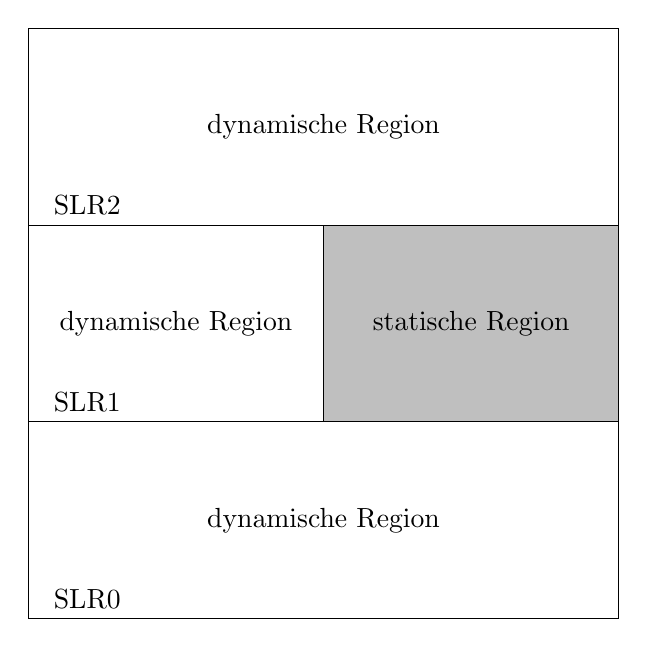
\begin{tikzpicture}
        % unten
        \draw (0.0, 0.0) rectangle (7.5, 2.5)
            node [pos = 0.5] {dynamische Region}
            node [pos = 0.1] {SLR0};

        % Mitte
        \draw [draw = none] (0.0, 2.5) rectangle (7.5, 5)
            node [pos = 0.1] {SLR1};
        \draw (0.0, 2.5) rectangle (3.75, 5)
            node [pos = 0.5] {dynamische Region};
        \draw [fill = lightgray] (3.75, 2.5) rectangle (7.5, 5)
            node [pos = 0.5] {statische Region};

        % oben
        \draw (0.0, 5) rectangle (7.5, 7.5)
            node [pos = 0.5] {dynamische Region}
            node [pos = 0.1] {SLR2};
    \end{tikzpicture}
    \caption{Aufbau eines XCU200-FPGAs \cite[nach][5]{alveo2019}}
    \label{fpga:aufbau:alveoslr}
\end{figure}

\begin{table}[htb]
    \centering
    \begin{tabulary}{\textwidth}{@{}LCCCC@{}}
        \toprule
        \textbf{Ressource} & \textbf{Gesamt} & \textbf{SLR0} & \textbf{SLR1}
            & \textbf{SLR2} \tabularnewline\midrule
        \textit{Configurable logic blocks (CLBs)}
            \tablefootnote{Xilinx macht
            in seinen Datenblättern keine Angaben zur Anzahl der CLBs auf
            dem XCU200-FPGA. Die Zahl der CLBs wurde daher rechnerisch aus
            der Zahl der \textit{look-up tables} (LUT) bestimmt, die in den
            Datenblättern angegeben wird. Die UltraScale-Architektur bildet
            aus jeweils acht LUTs einen CLB
            \cite[siehe][38]{ultrascale2019}.} & \num{111500} &
            \num{45625} & \num{20250} & \num{45625}\tabularnewline
        Register & \num{1831000} & \num{746000} & \num{339000} & 
            \num{746000}\tabularnewline
        Block-RAM (\SI{36}{\kibi\byte}) & \num{1766} & \num{695} & 
            \num{376} & \num{695}\tabularnewline
        UltraRAM (\SI{288}{\kibi\byte}) & \num{800} & \num{320} &
            \num{160} & \num{320}\tabularnewline
        DSP-Schichten & \num{5867} & \num{2275} & \num{1317} &
            \num{2275}\tabularnewline\bottomrule
    \end{tabulary}
    \caption{Ressourcen der dynamischen Regionen eines XCU200-FPGAs
             \cite[siehe][5]{alveo2019}}
    \label{fpga:aufbau:ressourcen}
\end{table}


\cite{ultrascale2019}

Alveo U200
\begin{itemize}
    \item drei \textit{super logic regions} (SLRs)
    \item entspricht drei dynamischen Regionen (vom Benutzer programmierbar) und
          einer statischen Region (deployment shell für Konfiguration)
    \item SLR0, SLR2: 365K LUTs, 746K Register, 695 36KB block RAM, 320 288Kb UltraRAM, 2275 DSPs
    \item SLR1: 162K LUTs, 339K Register, 376KB block RAM, 160 288Kb UltraRAM, 1317 DSPs
\end{itemize}

LUT
\begin{itemize}
    \item 45625 Configurable Logic Blocks (CLBs) à 8 LUTs und 16 flip-flops (SLR0, SLR2) bzw. 20250 CLBs (SLR1)
    \item demnach 730000 flip-flops (SLR0, SLR2) bzw. 324000 flip-flops (SLR1)
    \item CLB enthält Logik für arithmetischen Übertrag und Multiplexer, dadurch komplexere Logikfunktionen möglich, sowie Kontrollsignale
    \item CLB sind über verschiedene Verbindungspfade verbunden, die 1, 2, 4, 5, 12 oder 16 CLBs miteinander verbinden
\end{itemize}

Register -- TODO

block RAM
\begin{itemize}
    \item jeder 36Kb Block hat zwei unabhängige Ports, die sich die Daten im Block teilen
    \item kann als 1 36Kb Block oder als 2 18Kb Blöcke konfiguriert werden
    \item Ports haben programmierbare Datenbreite: 32K x 1, 16K x 2, 8K x 4, 4K x 9 (oder 8), 2K x 18 (oder 16), 1K x 36 (oder 32), 512 x 72 (oder 64)
    \item unterschiedliche Datenbreiten für die Ports möglich
    \item ECC unterstützt
    \item als FIFO konfigurierbar
    \item vertikal nebeneinander liegende Blocks lassen sich verbinden, wodurch größere Speicherbereiche entstehen
\end{itemize}

UltraRAM
\begin{itemize}
    \item jeder 288Kb UltraRAM hat zwei unabhängige Ports
    \item feste Datenbreite: 4K x 72
    \item UltraRAM-Spalten lassen sich verbinden, so sind bis zu 100MB möglich
\end{itemize}

DSP
\begin{itemize}
    \item spezielle Funktionseinheiten, die für Signalverarbeitung optimiert sind
    \item enthalten 27 x 18 bit Multiplizierern (Zweierkomplement) und einen 48-bit Akkumulator
    \item Multiplizierer kann überbrückt werden
    \item zwei 48-bit Eingaben können eine SIMD-Einheit füttern (2x 24-bit Addition / Subtraktion / Akkumulation oder 4x 12-bit Addition / ...) oder aber eine Logik-Einheit, die bis zu zehn verschiedene Logikfunktionen für beide Operanden generieren kann
    \item enthält Voraddierer (symmetrische Filter)
    \item 96-bit XOR-Funktion, programmierbar auf 12, 24, 48 oder 96 bit
    \item 48-bit Muster-Detektor, kann mit der Logikeinheit verbunden werden, um Logikfunktionen mit 96-bit Breite zu generieren
    \item eignet sich für Pipelining und Anwendungen außerhalb der DSP
\end{itemize}

\subsection{Anwendungsfälle}

Gegenüber ASICs bieten \gls{fpga}s einige Vorteile. Da sich Schaltungen ohne
einen Produktionsprozess schneller in Hardware abbilden lassen, eignen sich
\gls{fpga}s für die Entwicklung neuer Schaltungen durch die Methode des
\textit{rapid prototyping} und damit für eine schnellere Markteinführung. Durch
die einfache Neuprogrammierung lassen sich Fehler außerdem während des
Entwicklungsprozesses sowie während des Lebenszyklus des Produkts deutlich
einfacher beheben, als dies bei ASICs der Fall wäre.
\cite[vgl.][10-1]{hawkins2010}

Dadurch eignen sich \gls{fpga}s sehr gut für den Einsatz als Schaltkreise, die
in kleiner bis mittlerer Menge produziert werden sollen, weil die finanzielle
Einstiegshürde deutlich geringer als bei ASICs ist. Umgekehrt sind ASICs bei
hohen Produktionsvolumen überlegen, da die Kosten pro Chip geringer sind.
\cite[vgl.][10-2]{hawkins2010}

In jüngerer Zeit wurden \gls{fpga}s auch außerhalb des klassischen
Schaltkreisentwurfs eingesetzt. So setzt die Firma Microsoft beispielsweise
\gls{fpga}s des Herstellers Intel für die Inferenz tiefer neuraler Netzwerke
\cite[vgl.][]{fowers2018, chung2018} sowie als besonders schnelle
Netzwerkkarten ein \cite[vgl.][]{firestone2018}.

\section{Entwicklungsprozess}

\subsection{Hardware-Beschreibungssprachen}

\subsection{High-Level-Synthese}

\section{Parallelität}
